\section{Ergebnisse}
\label{ergebnisse}

Dieses Kapitel stellt die Ergebnisse einer ausgewählten Untermenge der in dieser Arbeit vorgestellten Graphrepräsentationen von Bildern, den Ansätzen zum Lernen auf diesen sowie den beschriebenen Datensätzen und Superpixelalgorithmen vor.
Zur Kenntlichmachung der einzelnen Ansätze erhält der weiterentwickelte Ansatz des räumlichen Lernens auf Graphen (\vgl{} Kapitel~\ref{raeumliches_lernen}) die Abkürzung \enquote{\acs{RL}} und das spektrale Lernen auf Graphen über den Tschebyschow-Polynomen (\vgl{} Kapitel~\ref{spektraler_faltungsoperator}) \bzw{} dessen Einschränkung auf eine Filtergröße von Eins (\vgl{} Kapitel~\ref{graph_convolutional_networks}) die Abkürzungen \enquote{\acs{SGCNN}} \bzw{} \enquote{\acs{GCN}}~\cite{patchy, Defferrard, gcn}.
Der in dieser Arbeit weiterentwickelte Ansatz zum spektralen Lernen ist über \enquote{\acs{EGCNN}} gekennzeichnet (\vgl{} Kapitel~\ref{gcn_erweiterung}).
Alle Faltungen des \acs{EGCNN}s wurden dabei mit einer Partitionsgröße von $8$ bei einem Grad von Eins implementiert, um ein \gls{CNN} mit einem $3 \times 3$ Filter zu simulieren.

Netzarchitekturen werden im Folgenden \bspw{} über ein Muster der Form \enquote{C32-P2-FC128} beschrieben und signalisieren eine Faltungsschicht, die auf 32 Merkmalskarten abbildet, gefolgt von einer Poolingschicht, welche zwei Knoten vereint, und danach mit einer vollverbundenen Schicht zu 128 Neuronen verknüpft wird.
Die für das spektrale Lernen bei dynamischen Eingabegrößen notwendige Durchschnittsbildung zwischen Faltungs- und vollverbundener Schicht wird als \enquote{Avg} gekennzeichnet (\vgl{} Kapitel~\ref{spektrale_netzarchitektur}).
Auf die explizite Erwähnung der Eingabe- und Ausgabeschichten der Netze wird übersichtshalber verzichtet.

\paragraph{\gls{MNIST}}

Zur Valdierung der Faltungansätze im Vergleich zur klassischen Faltungsoperation eignet sich die in Kapitel~\ref{gitter} beschriebene Graphrepräsentation der Bilder über ein reguläres Gitter, da diese anstelle der Bilder eine äquivalente Eingabe in das Netz darstellen.
Damit verfällt insbesondere die Notwendigkeit die Anwendung der Durchschnittsbildung, da die Anzahl an Neuronen zu jedem Zeitpunkt klar definiert ist.
Für das räumliche Lernen werden dabei 196 Knoten mit Schrittweite 4 bei $\delta=1$ und einer Nachbarschaftsgröße von 25 ausgewählt (\vgl{} Kapitel~\ref{raeumliches_lernen}).
Die Graphvergröberung des spektralen Lernens wiederum generiert für die erste Schicht 976 Knoten ($28^2 = 784$ Pixelknoten und 192 Fakeknoten).
Die Anzahl der generierten Fakeknoten kann jedoch aufgrund der zufälligen Permutation variieren.
Tabelle~\ref{tab:train_mnist_gitter} fasst die Netzarchitekturen und dessen erreichte Genauigkeiten der einzelnen Ansätze zusammen.
\begin{table}[t]
\centering
\begin{tabular}{lclrr}
  \toprule
  Ansatz & \ma{W} & Architektur & Genauigkeit [\%]\\
  \midrule
  \acs{RL} & 25 & C64-FC1024 & 98.774 \\
  \acs{SGCNN} & 25 & C32-P4-C64-P4-FC1024 & 98.888\\
  \acs{GCN} & 1 & C32-C32-P4-C64-C64-P4-FC1024 & 96.675\\
  \acs{EGCNN} & 9 & C32-C32-P4-C64-C64-P4-FC1024 & 99.145\\
  \midrule
  klassisch & $5 \times 5$ & C32-P4-C64-P4-FC1024 & 99.189\\
  klassisch & $3 \times 3$ & C32-C32-P4-C64-C64-P4-FC1024 & 99.139\\
  \bottomrule
\end{tabular}
\caption[Testgenauigkeiten der \gls{MNIST}-Gitterrepräsentation]{Testgenauigkeiten der trainierten Netze auf einer \gls{MNIST}-Gitterrepräsentation nach 10 Epochen für die vorgestellten Ansätze inklusive äquivalenter Netzarchitekturen bei Benutzung der klassischen Faltungsoperation.
Die Spalte \ma{W} kennzeichnet die benutzten Filtergrößen der einzelnen Faltungsschichten.}
\label{tab:train_mnist_gitter}
\end{table}
Die Netzarchitekturen sind dabei an der von \texttt{tensorflow} vorgeschlagenen Architektur orientiert~\cite{tensorflow}.
Alle Netze wurden einheitlich mit einer Lernrate von $0.001$ über den \emph{Adam}-Optimierer trainiert~\cite{adam}.
Es wurde auf die für \gls{MNIST} eher untypische Augmentierung der Eingabedaten, die L2-Regularisierung sowie auf die Verminderung der Lernrate in Abhängigkeit zur Trainingsdauer ver\-zich\-tet~\cite{tensorflow}.
Es findet sich jedoch die Anwendung eines Dropouts von $0.5$ vor der Ausgabeschicht.
\citeauthor{Defferrard} benutzen zur Validierung des \acs{SGCNN}s eine ähnliche Netzarchitektur auf \gls{MNIST} und schlagen dazu eine Filtergröße von $25$ vor, sodass die Anzahl der Parameter mit der Anzahl der klassischen Faltung über ein $5 \times 5$ Fenster korrespondiert~\cite{Defferrard}.
Diese Faltung lässt sich im Kontext des spektralen Faltungsoperators auf einem Gitter der Größe $28 \times 28$ aber kaum noch als lokale Faltung verstehen, denn sie lässt Knoten in die Berechnung mit einfließen, die 25 Kanten weit vom Ursprungsknoten entfernt liegen, und betrachtet folglich außer bei Randknoten das globale Bild (\vgl{} Kapitel~\ref{spektraler_faltungsoperator}).
Eine lokalere Faltung lässt sich mit dem \acs{RL}, \acs{GCN} und \acs{EGCNN} gewinnen.
Für das \acs{GCN} zeigt sich dabei jedoch eine eindeutige Limitierung durch die geringe Filtergröße.
Die entwickelten Faltungsansätze \acs{RL} und \acs{EGCNN} beweisen sich aufgrund der Berücksichtigung ihrer Kantenausrichtungen als die bessere Alternative.
Insbesondere lässt sich die Äquivalenz des \acs{EGCNN}s \bzgl{} regulärer Gitter verifizieren.
Das räumliche Lernen zeigt sich aufgrund der Beschränkung auf eine Faltungsschicht, der eindimensionalen Knotenauswahl sowie der uneinheitlichen Nachbarschaftsanordnung an Randknoten als leicht schwächer.

Die in Tabelle~\ref{tab:train_mnist} vorgestellten Netzarchitekturen zeigen die Genauigkeiten des Trainings auf irregulären Dateneingaben, welche über die Superpixelalgorithmen \gls{SLIC} und \gls{QS} anhand der in Kapitel~\ref{datensaetze} vorgestellten Parameterwerte gewonnen wurden.
\begin{table}[t]
\centering
\begin{tabular}{lclrrr}
  \toprule
  Ansatz & \ma{W} & Architektur & \multicolumn{2}{c}{Genauigkeit [\%]}\\
  \cmidrule{4-5}
   & & & \acs{SLIC} & \acs{QS}\\
  \midrule
  \acs{RL} & 25 & C64-FC1024 & 82.873 & 85.226 \\
  \acs{SGCNN} & 9 & C64-P4-C128-P4-Avg & 91.884 & 92.718 \\
  \acs{GCN} & 1 & C64-C64-P4-C128-C128-P4-Avg & 78.155 & 86.358 \\
  \acs{EGCNN} & 9 & C64-C64-P4-C128-C128-P4-Avg & 97.405 & 98.025 \\
  \bottomrule
\end{tabular}
\caption[Testgenauigkeiten der \gls{MNIST} Superpixelrepräsentationen]{Testgenauigkeiten der trainierten Netze auf dem \gls{MNIST} Datensatz nach 17 Epochen, dessen Bilder zuvor durch die Superpixelalgorithmen \gls{SLIC} und Quickshift in irreguläre Graphrepräsentationen gebracht werden.}
\label{tab:train_mnist}
\end{table}
Bei \acs{SGCNN} wurde dabei aufgrund der reduzierten Datenmenge die Filtergröße im Vergleich zum Vortest gedrosselt und besitzt im Vergleich zu den \acs{GCN}- \bzw{} \acs{EGCNN}-Netzarchitekturen nicht mehrere, aufeinanderfolgende Faltungsschichten.

Es zeigt sich, dass alle Netzansätze auf irregulären Daten gar nicht oder nur knapp an die Ergebnisse auf regulären Gittereingaben heranreichen.
Insbesondere offenbart der räumliche Faltungsansatz hier seine Schwächen, denn obwohl die Trainingsmenge erfolgreich gelernt wird, so lässt sich auf unbekannte Eingaben aufgrund der Anordnung zu eindimensionalen Knoten- sowie Nachbarschaftsmengen für irreguläre Graphen nur schwer bis gar nicht generalisieren.
Für alle Ansätze zeigt sich des Weiteren die Quickshift-Segmentierung aufgrund ihrer überlegenden Segmentierung auf den Bildern des \gls{MNIST} Datensatz als die bessere Wahl (\vgl{} Abbildung~\ref{fig:mnist}).
Insbesondere erreicht der entwickelte spektrale Faltungsoperator über B-Spline-Kurven (\acs{EGCNN}) auch hier die eindeutig besten Resultate.

\paragraph{\gls{Cifar}-10}

Die Klassifikation auf dem \gls{Cifar}-10 Datensatz ist im Vergleich zu \gls{MNIST} eine anspruchsvollere Aufgabe, die insbesondere eine längere Trainingsdauer über weitaus mehr Epochen in Anspruch nimmt.
Wichtige Maßnahmen für qualitativ hochwertige Ergebnisse sind dabei insbesondere die in Kapitel~\ref{augmentierung} vorgestellten Augmentierungschritte der Eingabedaten~\cite{tensorflow}.
Es hat sich auch in der Evaluierung bewahrheitet, dass eine Augmentierung auf den Graphen schwächere Resultate als eine Augmentierung auf den Rohdaten des Bildes liefert und ein Genauigkeitsverlust von bis zu 5\% nach sich zieht.
Für alle Lernansätze wurden deshalb die Eingaben des \gls{Cifar}-10 Datensatz zur Laufzeit augmentiert und erst anschließend in eine Graph\-re\-prä\-sen\-ta\-tion transformiert.
Die Lernrate wurde dabei mit $0.001$ initialisiert und alle 6 Epochen exponentiell um $0.96$ verringert.
In den vollverbundenen Schichten, außer der Ausgabeschicht, besitzen die Gewichte \bzgl{} der L2-Regularisierung eine Dämpfungskonstante von $0.004$.
Vor der Ausgabeschicht sorgt die zusätzliche Anwendung eines Dropouts von $0.5$ dafür, ein Overfitting der Netze weiter zu vermeiden.
Tabelle~\ref{tab:train_cifar_10} fasst die Netzarchitekturen der einzelnen Ansätze und ihre erreichten Genauigkeiten nach rund 80 Epochen zusammen.
\begin{table}[t]
\centering
\resizebox{\textwidth}{!}{%
\begin{tabular}{lclrrr}
  \toprule
  Ansatz & \ma{W} & Architektur & \multicolumn{2}{c}{Genauigkeit [\%]}\\
  \cmidrule{4-5}
   & & & \acs{SLIC} & \acs{QS}\\
  \midrule
  \acs{SGCNN} & 9 & C64-P2-C128-P2-C256-P2-C512-Avg-FC256-FC128 & 66.814 & 67.748\\
  \acs{GCN} & 1 & C64-C64-P2-C128-P2-C256-P2-C512-Avg-FC256-FC128 & 54.497 & 53.606\\
  \acs{EGCNN} & 9 & C64-C64-P2-C128-P2-C256-P2-C512-Avg-FC256-FC128 & 74.218 & 75.230\\
  \midrule
  klassisch & $3 \times 3$ & C64-C64-P4-C128-P4-C256-P4-FC256-FC128 & \multicolumn{2}{c}{82.061} \\
  \bottomrule
\end{tabular}}
\caption[Testgenauigkeiten der \gls{Cifar}-10 Superpixelrepräsentationen]{Testgenauigkeiten der trainierten Netze auf den durch \gls{SLIC} und Quickshift zur Laufzeit generierten Graphrepräsentationen des \gls{Cifar}-10 Datensatz nach 80 Epochen im Vergleich zu einer ähnlichen klassischen Netzarchitektur auf den Bildrohdaten.}
\label{tab:train_cifar_10}
\end{table}
Alle spektralen Graphansätze auf den aus \gls{SLIC} und Quickshift generierten Graphrepräsentationen können nicht mit einer ähnlichen klassischen Netzarchitektur auf den Bildrohdaten konkurrieren.
Wohingegen jedoch die vorhandenen Ansätze \acs{SGCNN} und \acs{GCN} eine maximale Genauigkeit von rund 67\% erreichen, zeigt sich auch hier eine signfikante Verbesserung durch den neu entwickelten spektralen Faltungsoperator \acs{EGCNN}.
Er erreicht mit $75\%$ mittels der Quickshift-Segmentierung das beste Resultat.
Hochoptimierte Ansätze, bei denen noch weitaus mehr Augmentierungsschritte zum Einsatz kommen, erreichen auf \gls{Cifar}-10 jedoch bereits mehr als $90\%$ und so ist nicht auszuschließen, dass auch für \acs{EGCNN} weiterhin Potential nach oben besteht~\cite{fracmaxpool}.

Abbildung~\ref{fig:cifar_10_train} illustriert den Genauigkeitsverlauf des \gls{Cifar}-10 Trainings- und Validierungsdatensatzes in Abhängigkeit der vergangenen Epochen.
\begin{figure}[t]
\centering
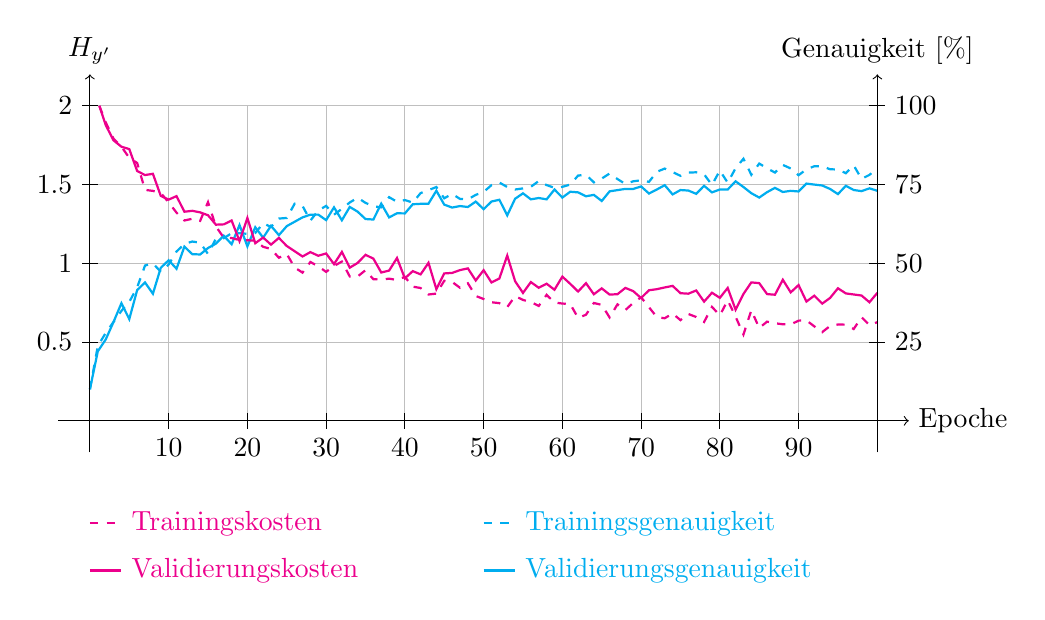
\begin{tikzpicture}
  \draw[color=lightgray] (0, 0) grid (10, 4);

  \tikzstyle{color1}=[color=cyan]
  \tikzstyle{color2}=[color=magenta]

  % Train accuracy.
  \draw[color1, dashed, thick] (0, 0.4) -- (0.1, 0.95) -- (0.2, 1.1146) -- (0.3, 1.2557) -- (0.4, 1.3958) -- (0.5, 1.5104) -- (0.6, 1.6944) -- (0.7, 1.9722) -- (0.8, 2.0) -- (0.9, 1.892) -- (1.0, 1.9844) -- (1.1, 2.15) -- (1.2, 2.2452) -- (1.3, 2.2768) -- (1.4, 2.2625) -- (1.5, 2.1181) -- (1.6, 2.3125) -- (1.7, 2.3188) -- (1.8, 2.3828) -- (1.9, 2.3819) -- (2.0, 2.375) -- (2.1, 2.3854) -- (2.2, 2.5089) -- (2.3, 2.4615) -- (2.4, 2.5682) -- (2.5, 2.5764) -- (2.6, 2.7569) -- (2.7, 2.7292) -- (2.8, 2.5417) -- (2.9, 2.6711) -- (3.0, 2.7292) -- (3.1, 2.6172) -- (3.2, 2.6927) -- (3.3, 2.7727) -- (3.4, 2.8333) -- (3.5, 2.7679) -- (3.6, 2.725) -- (3.7, 2.7109) -- (3.8, 2.8403) -- (3.9, 2.7812) -- (4.0, 2.8036) -- (4.1, 2.7708) -- (4.2, 2.892) -- (4.3, 2.9297) -- (4.4, 2.9688) -- (4.5, 2.8259) -- (4.6, 2.8819) -- (4.7, 2.8182) -- (4.8, 2.8125) -- (4.9, 2.8693) -- (5.0, 2.9062) -- (5.1, 2.9931) -- (5.2, 3.026) -- (5.3, 2.9688) -- (5.4, 2.9375) -- (5.5, 2.9514) -- (5.6, 2.9716) -- (5.7, 3.0455) -- (5.8, 2.9937) -- (5.9, 2.9583) -- (6.0, 2.9716) -- (6.1, 3.0) -- (6.2, 3.1146) -- (6.3, 3.125) -- (6.4, 3.0284) -- (6.5, 3.0764) -- (6.6, 3.1406) -- (6.7, 3.0703) -- (6.8, 3.0078) -- (6.9, 3.0417) -- (7.0, 3.0547) -- (7.1, 3.0341) -- (7.2, 3.1625) -- (7.3, 3.2031) -- (7.4, 3.1597) -- (7.5, 3.1111) -- (7.6, 3.1518) -- (7.7, 3.1562) -- (7.8, 3.1302) -- (7.9, 2.9948) -- (8.0, 3.1786) -- (8.1, 3.0234) -- (8.2, 3.2083) -- (8.3, 3.3281) -- (8.4, 3.125) -- (8.5, 3.267) -- (8.6, 3.2067) -- (8.7, 3.1528) -- (8.8, 3.25) -- (8.9, 3.2045) -- (9.0, 3.1187) -- (9.1, 3.1938) -- (9.2, 3.233) -- (9.3, 3.233) -- (9.4, 3.1944) -- (9.5, 3.1917) -- (9.6, 3.1445) -- (9.7, 3.2437) -- (9.8, 3.0729) -- (9.9, 3.123) -- (10, 3.208);

  % Validation accuracy.
  \draw[color1, thick] (0, 0.4) -- (0.1, 0.8812) -- (0.2, 1.0312) -- (0.3, 1.2557) -- (0.4, 1.4931) -- (0.5, 1.2917) -- (0.6, 1.6597) -- (0.7, 1.7569) -- (0.8, 1.6136) -- (0.9, 1.9432) -- (1.0, 2.0391) -- (1.1, 1.9312) -- (1.2, 2.2115) -- (1.3, 2.1161) -- (1.4, 2.1125) -- (1.5, 2.1944) -- (1.6, 2.25) -- (1.7, 2.35) -- (1.8, 2.2422) -- (1.9, 2.4861) -- (2.0, 2.2153) -- (2.1, 2.4583) -- (2.2, 2.3259) -- (2.3, 2.476) -- (2.4, 2.358) -- (2.5, 2.4722) -- (2.6, 2.5278) -- (2.7, 2.5833) -- (2.8, 2.6181) -- (2.9, 2.6184) -- (3.0, 2.5486) -- (3.1, 2.7109) -- (3.2, 2.5469) -- (3.3, 2.7159) -- (3.4, 2.6562) -- (3.5, 2.5625) -- (3.6, 2.5562) -- (3.7, 2.7578) -- (3.8, 2.5833) -- (3.9, 2.6354) -- (4.0, 2.6339) -- (4.1, 2.75) -- (4.2, 2.7557) -- (4.3, 2.7578) -- (4.4, 2.9219) -- (4.5, 2.7455) -- (4.6, 2.7083) -- (4.7, 2.7273) -- (4.8, 2.7153) -- (4.9, 2.7841) -- (5.0, 2.6875) -- (5.1, 2.7847) -- (5.2, 2.8073) -- (5.3, 2.6094) -- (5.4, 2.8203) -- (5.5, 2.8889) -- (5.6, 2.8125) -- (5.7, 2.8295) -- (5.8, 2.8125) -- (5.9, 2.9375) -- (6.0, 2.8352) -- (6.1, 2.9091) -- (6.2, 2.901) -- (6.3, 2.8516) -- (6.4, 2.8693) -- (6.5, 2.7917) -- (6.6, 2.9141) -- (6.7, 2.9297) -- (6.8, 2.9453) -- (6.9, 2.9444) -- (7.0, 2.9766) -- (7.1, 2.8864) -- (7.2, 2.9375) -- (7.3, 2.9922) -- (7.4, 2.875) -- (7.5, 2.9306) -- (7.6, 2.9241) -- (7.7, 2.8828) -- (7.8, 2.9844) -- (7.9, 2.901) -- (8.0, 2.9375) -- (8.1, 2.9375) -- (8.2, 3.0417) -- (8.3, 2.9688) -- (8.4, 2.8906) -- (8.5, 2.8352) -- (8.6, 2.9038) -- (8.7, 2.9583) -- (8.8, 2.9062) -- (8.9, 2.9205) -- (9.0, 2.9125) -- (9.1, 3.0125) -- (9.2, 3.0) -- (9.3, 2.9886) -- (9.4, 2.9444) -- (9.5, 2.8792) -- (9.6, 2.9844) -- (9.7, 2.9312) -- (9.8, 2.9167) -- (9.9, 2.9523) -- (10, 2.9214);

  % Train loss.
  \draw[color2, dashed, thick] (0.12, 4) -- (0.2, 3.7924) -- (0.3, 3.5816) -- (0.4, 3.4817) -- (0.5, 3.339) -- (0.6, 3.2744) -- (0.7, 2.933) -- (0.8, 2.92) -- (0.9, 2.893) -- (1.0, 2.7748) -- (1.1, 2.6434) -- (1.2, 2.5438) -- (1.3, 2.566) -- (1.4, 2.5388) -- (1.5, 2.7772) -- (1.6, 2.4688) -- (1.7, 2.3255) -- (1.8, 2.3209) -- (1.9, 2.2951) -- (2.0, 2.2934) -- (2.1, 2.2871) -- (2.2, 2.2098) -- (2.3, 2.182) -- (2.4, 2.0707) -- (2.5, 2.1185) -- (2.6, 1.9472) -- (2.7, 1.882) -- (2.8, 2.017) -- (2.9, 1.962) -- (3.0, 1.8913) -- (3.1, 1.9663) -- (3.2, 2.0222) -- (3.3, 1.8329) -- (3.4, 1.833) -- (3.5, 1.9122) -- (3.6, 1.7979) -- (3.7, 1.7941) -- (3.8, 1.8049) -- (3.9, 1.7891) -- (4.0, 1.8278) -- (4.1, 1.7039) -- (4.2, 1.6864) -- (4.3, 1.6041) -- (4.4, 1.6157) -- (4.5, 1.7782) -- (4.6, 1.7638) -- (4.7, 1.6894) -- (4.8, 1.7469) -- (4.9, 1.5853) -- (5.0, 1.547) -- (5.1, 1.5054) -- (5.2, 1.4945) -- (5.3, 1.4434) -- (5.4, 1.5836) -- (5.5, 1.5352) -- (5.6, 1.5082) -- (5.7, 1.4586) -- (5.8, 1.5991) -- (5.9, 1.5021) -- (6.0, 1.4892) -- (6.1, 1.483) -- (6.2, 1.307) -- (6.3, 1.3468) -- (6.4, 1.4963) -- (6.5, 1.4723) -- (6.6, 1.3129) -- (6.7, 1.4788) -- (6.8, 1.4064) -- (6.9, 1.4973) -- (7.0, 1.5687) -- (7.1, 1.4423) -- (7.2, 1.317) -- (7.3, 1.3022) -- (7.4, 1.3634) -- (7.5, 1.2786) -- (7.6, 1.3565) -- (7.7, 1.3183) -- (7.8, 1.2549) -- (7.9, 1.447) -- (8.0, 1.3388) -- (8.1, 1.5304) -- (8.2, 1.3225) -- (8.3, 1.0959) -- (8.4, 1.4044) -- (8.5, 1.1791) -- (8.6, 1.2593) -- (8.7, 1.2394) -- (8.8, 1.2256) -- (8.9, 1.2238) -- (9.0, 1.2721) -- (9.1, 1.2754) -- (9.2, 1.1993) -- (9.3, 1.1261) -- (9.4, 1.2046) -- (9.5, 1.2231) -- (9.6, 1.2211) -- (9.7, 1.1656) -- (9.8, 1.3159) -- (9.9, 1.2148) -- (10, 1.2526);

  % Validation loss.
  \draw[color2, thick] (0.12, 4) -- (0.2, 3.7574) -- (0.3, 3.5618) -- (0.4, 3.4812) -- (0.5, 3.4506) -- (0.6, 3.1727) -- (0.7, 3.121) -- (0.8, 3.137) -- (0.9, 2.8564) -- (1.0, 2.8091) -- (1.1, 2.8534) -- (1.2, 2.6553) -- (1.3, 2.6668) -- (1.4, 2.6473) -- (1.5, 2.6105) -- (1.6, 2.4908) -- (1.7, 2.4949) -- (1.8, 2.5435) -- (1.9, 2.2812) -- (2.0, 2.5756) -- (2.1, 2.2554) -- (2.2, 2.3275) -- (2.3, 2.2373) -- (2.4, 2.3227) -- (2.5, 2.22) -- (2.6, 2.1535) -- (2.7, 2.087) -- (2.8, 2.1421) -- (2.9, 2.0962) -- (3.0, 2.1254) -- (3.1, 1.9896) -- (3.2, 2.1447) -- (3.3, 1.9447) -- (3.4, 2.0049) -- (3.5, 2.108) -- (3.6, 2.0597) -- (3.7, 1.8835) -- (3.8, 1.908) -- (3.9, 2.0677) -- (4.0, 1.8087) -- (4.1, 1.9008) -- (4.2, 1.8596) -- (4.3, 2.0063) -- (4.4, 1.6715) -- (4.5, 1.8716) -- (4.6, 1.8781) -- (4.7, 1.9138) -- (4.8, 1.9358) -- (4.9, 1.7821) -- (5.0, 1.9127) -- (5.1, 1.7567) -- (5.2, 1.8072) -- (5.3, 2.0986) -- (5.4, 1.7727) -- (5.5, 1.624) -- (5.6, 1.7619) -- (5.7, 1.6896) -- (5.8, 1.7412) -- (5.9, 1.6644) -- (6.0, 1.8309) -- (6.1, 1.7395) -- (6.2, 1.6417) -- (6.3, 1.748) -- (6.4, 1.607) -- (6.5, 1.6818) -- (6.6, 1.6032) -- (6.7, 1.6078) -- (6.8, 1.688) -- (6.9, 1.6468) -- (7.0, 1.5591) -- (7.1, 1.6582) -- (7.2, 1.6715) -- (7.3, 1.6938) -- (7.4, 1.7135) -- (7.5, 1.6207) -- (7.6, 1.6145) -- (7.7, 1.6552) -- (7.8, 1.5135) -- (7.9, 1.6266) -- (8.0, 1.562) -- (8.1, 1.6873) -- (8.2, 1.4112) -- (8.3, 1.611) -- (8.4, 1.7578) -- (8.5, 1.7484) -- (8.6, 1.6091) -- (8.7, 1.6011) -- (8.8, 1.7912) -- (8.9, 1.6309) -- (9.0, 1.724) -- (9.1, 1.5145) -- (9.2, 1.589) -- (9.3, 1.4882) -- (9.4, 1.5603) -- (9.5, 1.6832) -- (9.6, 1.6179) -- (9.7, 1.6045) -- (9.8, 1.591) -- (9.9, 1.5056) -- (10, 1.6248);

  \draw (0.1, 4) -- (-0.1, 4) node[left] {$2$};
  \draw (0.1, 3) -- (-0.1, 3) node[left] {$1.5$};
  \draw (0.1, 2) -- (-0.1, 2) node[left] {$1$};
  \draw (0.1, 1) -- (-0.1, 1) node[left] {$0.5$};

  \draw (9.9, 4) -- (10.1, 4) node[right] {$100$};
  \draw (9.9, 3) -- (10.1, 3) node[right] {$75$};
  \draw (9.9, 2) -- (10.1, 2) node[right] {$50$};
  \draw (9.9, 1) -- (10.1, 1) node[right] {$25$};

  \draw (1, 0.1) -- (1, -0.1)  node[below] {$10$};
  \draw (2, 0.1) -- (2, -0.1)  node[below] {$20$};
  \draw (3, 0.1) -- (3, -0.1)  node[below] {$30$};
  \draw (4, 0.1) -- (4, -0.1)  node[below] {$40$};
  \draw (5, 0.1) -- (5, -0.1)  node[below] {$50$};
  \draw (6, 0.1) -- (6, -0.1)  node[below] {$60$};
  \draw (7, 0.1) -- (7, -0.1)  node[below] {$70$};
  \draw (8, 0.1) -- (8, -0.1)  node[below] {$80$};
  \draw (9, 0.1) -- (9, -0.1)  node[below] {$90$};

  \draw[->] (-0.4, 0)    -- (10.4, 0)   node[right] {Epoche};
  \draw[->] (0,    -0.4) -- (0,    4.4) node[above] {$H_{y^{\prime}}$};
  \draw[->] (10,   -0.4) -- (10,   4.4) node[above] {Genauigkeit [\%]};

  \draw[color2, thick, dashed] (0, -1.3) -- (0.4, -1.3) node[right] {Trainingskosten};
  \draw[color2, thick]         (0, -1.9) -- (0.4, -1.9) node[right] {Validierungskosten};
  \draw[color1, thick, dashed] (5, -1.3) -- (5.4, -1.3) node[right] {Trainingsgenauigkeit};
  \draw[color1, thick]         (5, -1.9) -- (5.4, -1.9) node[right] {Validierungsgenauigkeit};

\end{tikzpicture}
\caption[\gls{Cifar}-10 Kosten- und Genauigkeitsverlauf]{Kosten- und Genauigkeitsverlauf eines Trainings auf dem \gls{Cifar}-10 Datensatz mit dem spektralen Faltungsoperator auf Graphen im zweidimensionalen euklidischen Raum, welche über Quickshift generiert wurden.
Die gestrichelten Linien zeigen die Kosten und Genauigkeiten des Trainingsdatensatzes in Abhängigkeit der Epochen, wohingegen die durchgezogenen Linien sich auf den Validierungsdatensatz beziehen.
Nach der $60$ten Epoche stellt sich eine deutliche Verlangsamung der Lerngeschwindigkeit ein.}
\label{fig:cifar_10_train}
\end{figure}

Wohingegen der klassische Ansatz recht schnell nach ungefähr 14 Epochen seine Maximalgenauigkeit erreicht und den Rest des Trainings damit verbringt, seine Gewichte auf die Trainingsdaten \enquote{überanzupassen}, ist zu beobachten, dass die Graphansätze weitaus langsamer und kontinuierlicher lernen.

\paragraph{\gls{Pascal}}

Für die Evaluierung der Ergebnisse auf dem \gls{Pascal} Datensatz wurde zum Vergleich die SqueezeNet-Architektur in Version 1.1 auf den Bildrohdaten zu Rate gezogen (\vgl{}~\cite{squeeze}).
Das SqueezeNet gilt aufgrund ihres Preis-Leistungs-Verhältnis zwischen ermittelter Genauigkeit und Anzahl zu trainierender Parameter als bewährte Netzarchiktektur für die Klassifizerung von Bildern mit recht hoher Auflösung~\cite{squeeze}.
Zur Verwendung wurden die Bilder dafür einheitlich auf die Größe $224 \times 224$ skaliert und mit schwarzen Bereichen an den horizontalen oder vertikalen Rändern je nach Ursprungsauflösung befüllt.
Für das Lernen auf Graphen ist diese Skalierung der Bildeingabedaten nicht von Nöten.
Die Klassen der Bilder wurden über das Objekt mit dem größten Hüllkörper bestimmt (\vgl{} Kapitel~\ref{datensaetze}).
Für die Netzarchitektur wurde dabei insbesondere im Vergleich zu vorherigen Testläufen auf die Verwendung mehrmaliger hintereinanderfolgender Faltungsschichten verzichtet.
Die Superpixel, die aus den Bildern von \gls{Pascal} generiert werden, sind bereits ausreichend groß und eine einzige Faltung auf diesen deckt bereits einen großen Bereich des Bildes ab.
Aus laufzeittechnischen Gründen findet das Training des Netzes ausschließlich auf vorverarbeiten Daten statt und erlaubt damit lediglich eine Augmentierung der Graphen anstelle der Bilder (\vgl{} Kapitel~\ref{laufzeitanalyse}).
Es finden sich weiterhin Anwendungen der Dropout-Technik und der L2-Regularisierung in den vollverbundenen Schichten bei einer Lernrate von 0.0001 für das SqueezeNet und 0.001 bei den Graphansätzen.

Tabelle~\ref{tab:train_pascal} stellt die Ergebnisse des SqueezeNets mit den Ergebnissen auf irregulären Dateneingaben bei Benutzung des \acs{EGCNN}s gegenüber.
\begin{table}[t]
\centering
\resizebox{\textwidth}{!}{%
\begin{tabular}{lclrrr}
  \toprule
  Ansatz & \ma{W} & Architektur & \multicolumn{2}{c}{Genauigkeit [\%]}\\
  \cmidrule{4-5}
   & & & \acs{SLIC} & \acs{QS}\\
  \midrule
  \acs{EGCNN} & 9 & C64-P2-C128-P2-C256-P2-C512-Avg-FC256-FC128 & 54.473 & 54.516\\
  \midrule
  klassisch & — & SqueezeNet 1.1 & \multicolumn{2}{c}{54.731} \\
  \bottomrule
\end{tabular}}
\caption[Testgenauigkeiten der \gls{Pascal} Superpixelrepräsentationen]{Testgenauigkeiten der trainierten Netze auf den durch \gls{SLIC} und Quickshift vorab generierten Graphrepräsentationen des \gls{Pascal} Datensatz nach 70 Epochen im Vergleich zu der Verwendung des SqueezeNets in Version 1.1 auf den Bildrohdaten~\cite{squeeze}.}
\label{tab:train_pascal}
\end{table}
Es zeigt sich, dass auf \gls{Pascal} die Graphansätze durchaus mit klassischen Lösungen auf diesem Gebiet mithalten können.
Sie beweisen sich als lediglich marginal schwächer gegenüber der Benutzung einer ausgereiften Architektur wie dem SqueezeNet.
Die allgemein relativ schwachen Ergebnisse sind damit unter Umständen auf die Transformation von \gls{Pascal} zu einem Klassfikationsdatensatz zurückzuführen.
Bilder, die mehrere Objekte enthalten, werden über die Größe ihrer Hüllkörper auf eine Objektklasse reduziert und verweisen damit nicht zwangsläufig auf das dominierende Objekt des Bildes.
Des Weiteren beinhaltet der Datensatz eine weitaus geringere Trainingsmenge als die Datensätze \gls{MNIST} und \gls{Cifar}-10.
